\documentclass[10pt]{beamer}

\usetheme[progressbar=frametitle]{metropolis}
\usepackage{appendixnumberbeamer}

\usepackage{booktabs}
\usepackage[scale=2]{ccicons}
\usepackage{xeCJK}
\usepackage{amsmath}

\usepackage{pgfplots}
\usepgfplotslibrary{dateplot}

\usepackage{xspace}
\usepackage[flushleft]{threeparttable}
\usepackage{caption,booktabs}
\newcommand{\themename}{\textbf{\textsc{metropolis}}\xspace}
\setbeamercolor{background canvas}{bg=white}
\title{Yelp Data Prediction}

% \date{\today}
\date{}
\author{Yifan Li, Chenlai Shi, Jianmin Chen}
\institute{Monday Group 1}
% \titlegraphic{\hfill\includegraphics[height=1.5cm]{logo.pdf}}

\begin{document}

\maketitle



\begin{frame}{1 Introduction and Data Cleaning}
\textbf{Introduction}
\begin{itemize}
	\item Small set of informative features
	\item Accurate predictive model
	\item Based on about 1.5 million Yelp reviews
\end{itemize}

\textbf{Data Cleaning}
\begin{itemize}
	\item Modify Abbreviation and Special Symbol

	\item Remove Non-English

	\item Negative Sentences
	
	\item Remove Punctuation
\end{itemize}
\end{frame}


%2---------------------------------------------------------------------------------------


\begin{frame}{2 Model: LSTM}

\textbf{Model}: Neural Network with 3 layers\\
\begin{itemize}
	\item layer1: LSTM layer with 50 output nodes
	\item layer2: Dense layer with 3 output nodes
	\item layer3: Dense layer with 1 output nodes
\end{itemize}

\centering
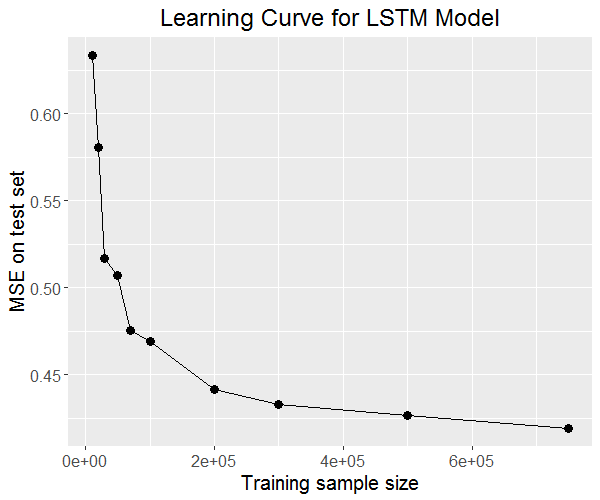
\includegraphics[scale=0.4]{../image/learning_curve.png}


\end{frame}




\begin{frame}{2.1 Pre-trained Sentence Vectores}
\textbf{Model Features}
\begin{itemize}
	\item Pre-trained Sentence Vectors: Capture word counts and order
	\item Additional  Variables: Capture sentiment, review date and location
\end{itemize}
\centering
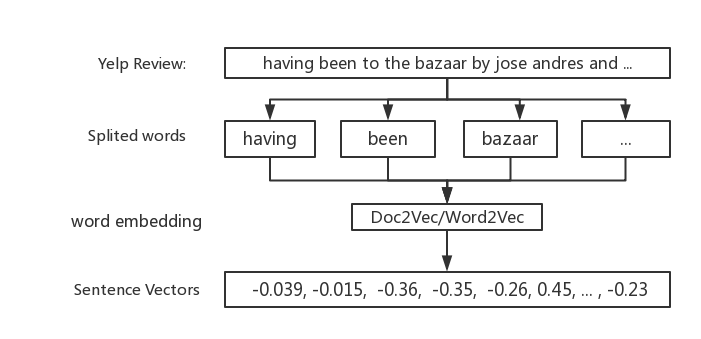
\includegraphics[scale=0.4]{../image/embedding.png}


\end{frame}


\begin{frame}{2.2 Additional Variables}

\begin{itemize}
	\item[-] \textbf{year}: scaled year variable.
	
	\item[-] \textbf{loc1}: 1 if the restaurant is in the Western United States, otherwise 0.
	
	\item[-] \textbf{loc2}: 1 if the restaurant is in the Eastern United States, otherwise 0.
	
\end{itemize}


\begin{figure}[htbp]
\centering
\begin{minipage}[t]{0.5\textwidth}
\centering
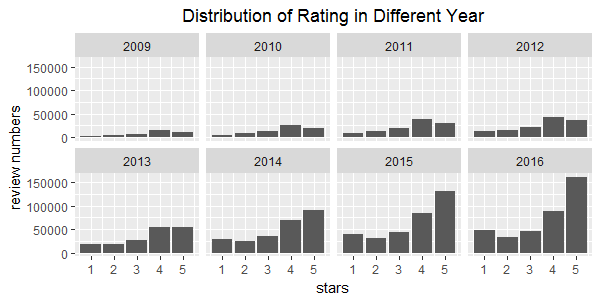
\includegraphics[width=5.4cm,height=2.7cm]{../image/year.png}

\end{minipage}
\begin{minipage}[t]{0.48\textwidth}
\centering
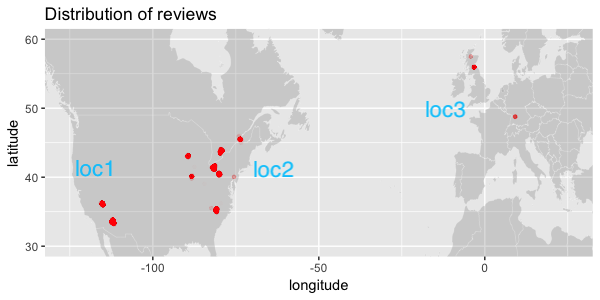
\includegraphics[width=5.4cm,height=2.7cm]{../image/worldmap.png}

\end{minipage}
\end{figure}

\end{frame}


\begin{frame}{2.2 Additional Variables}

\begin{itemize}
\item[-] \textbf{Score1$\sim$5}: Score1[word] = $\frac{\text{P(this word is included in reviews with 1-star)}}{\text{P(this word is included in reviews with other stars)}}$\\
\item[-] \textbf{S1 $\sim$ S5}: S1[review] = \# of words with high Score1 in the review.
\end{itemize}

\begin{table}[ht]

\centering % used for centering table
\begin{tabular}{l l r r r r r r} % centered columns (4 columns)
	\hline %inserts double horizontal lines
	Word   &Variable  & 1-star & 2-star & 3-star & 4-star & 5-star  \\ [0.5ex] % inserts table
	%heading
	\hline % inserts single horizontal line
	\textbf{refund}         & frequence   & 115    & 15     & 7      & 4      & 2      \\
	& probability & 0.011  & 0.002  & 0      & 0      & 0      \\
	& Score     & 34.200 & 1.080  & 0.300  & 0.072  & 0.025  \\
	\hline
	\textbf{notdisappoints} & frequence   & 0      & 2      & 5      & 43     & 110   \\
	& probability & 0      & 0      & 0      & 0.002  & 0.003  \\
	& Score     & 0      & 0.116  & 0.188  & 0.917  & 3.870  \\
	\hline
	\textbf{and}            & frequence   & 9196   & 8691   & 12851  & 25604  & 32071  \\
	& probability & 0.859  & 0.886  & 0.877  & 0.895  & 0.886  \\
	& Score     & 0.968  & 1.000  & 0.991  & 1.020  & 1.000  \\
	
	\hline %inserts single line
\end{tabular}
\label{table:nonlin} % is used to refer this table in the text
\end{table}

\end{frame}

\begin{frame}{2.2 Additional Variables}
\begin{figure}[htbp]
\centering
\begin{minipage}[t]{0.5\textwidth}
\centering
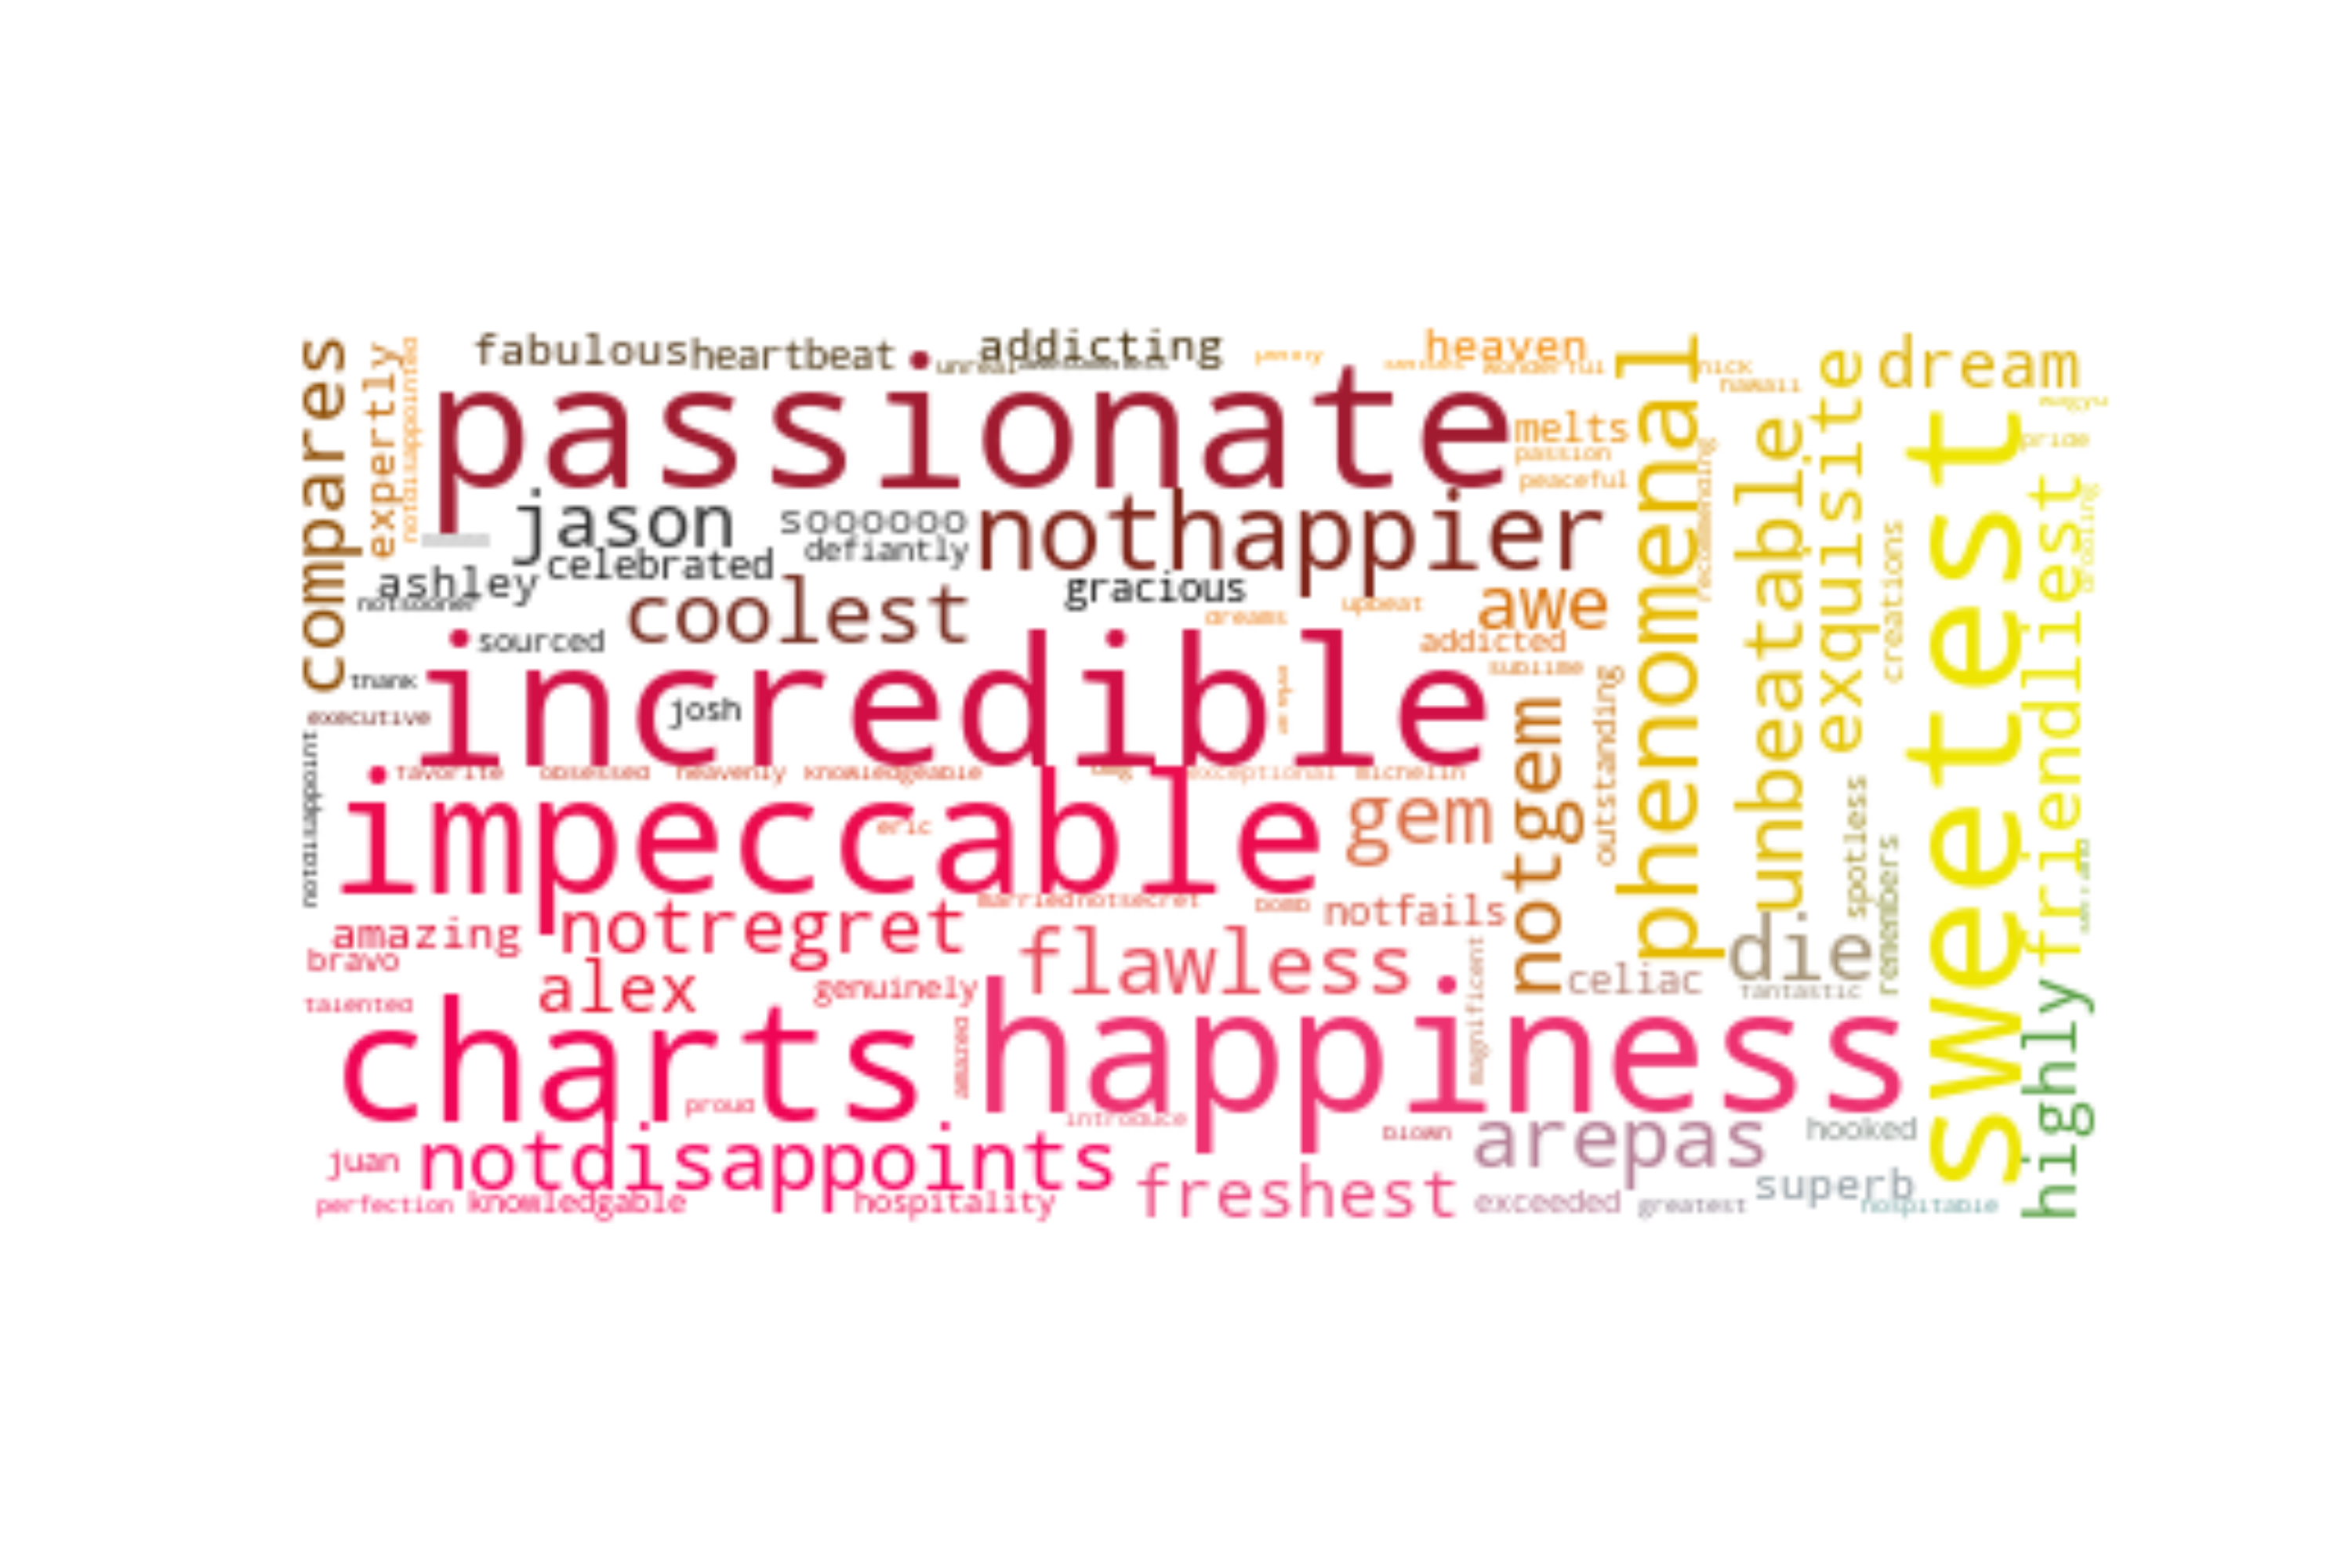
\includegraphics[width=4.8cm,height=5cm]{../image/dist5.png}

\end{minipage}
\begin{minipage}[t]{0.48\textwidth}
\centering
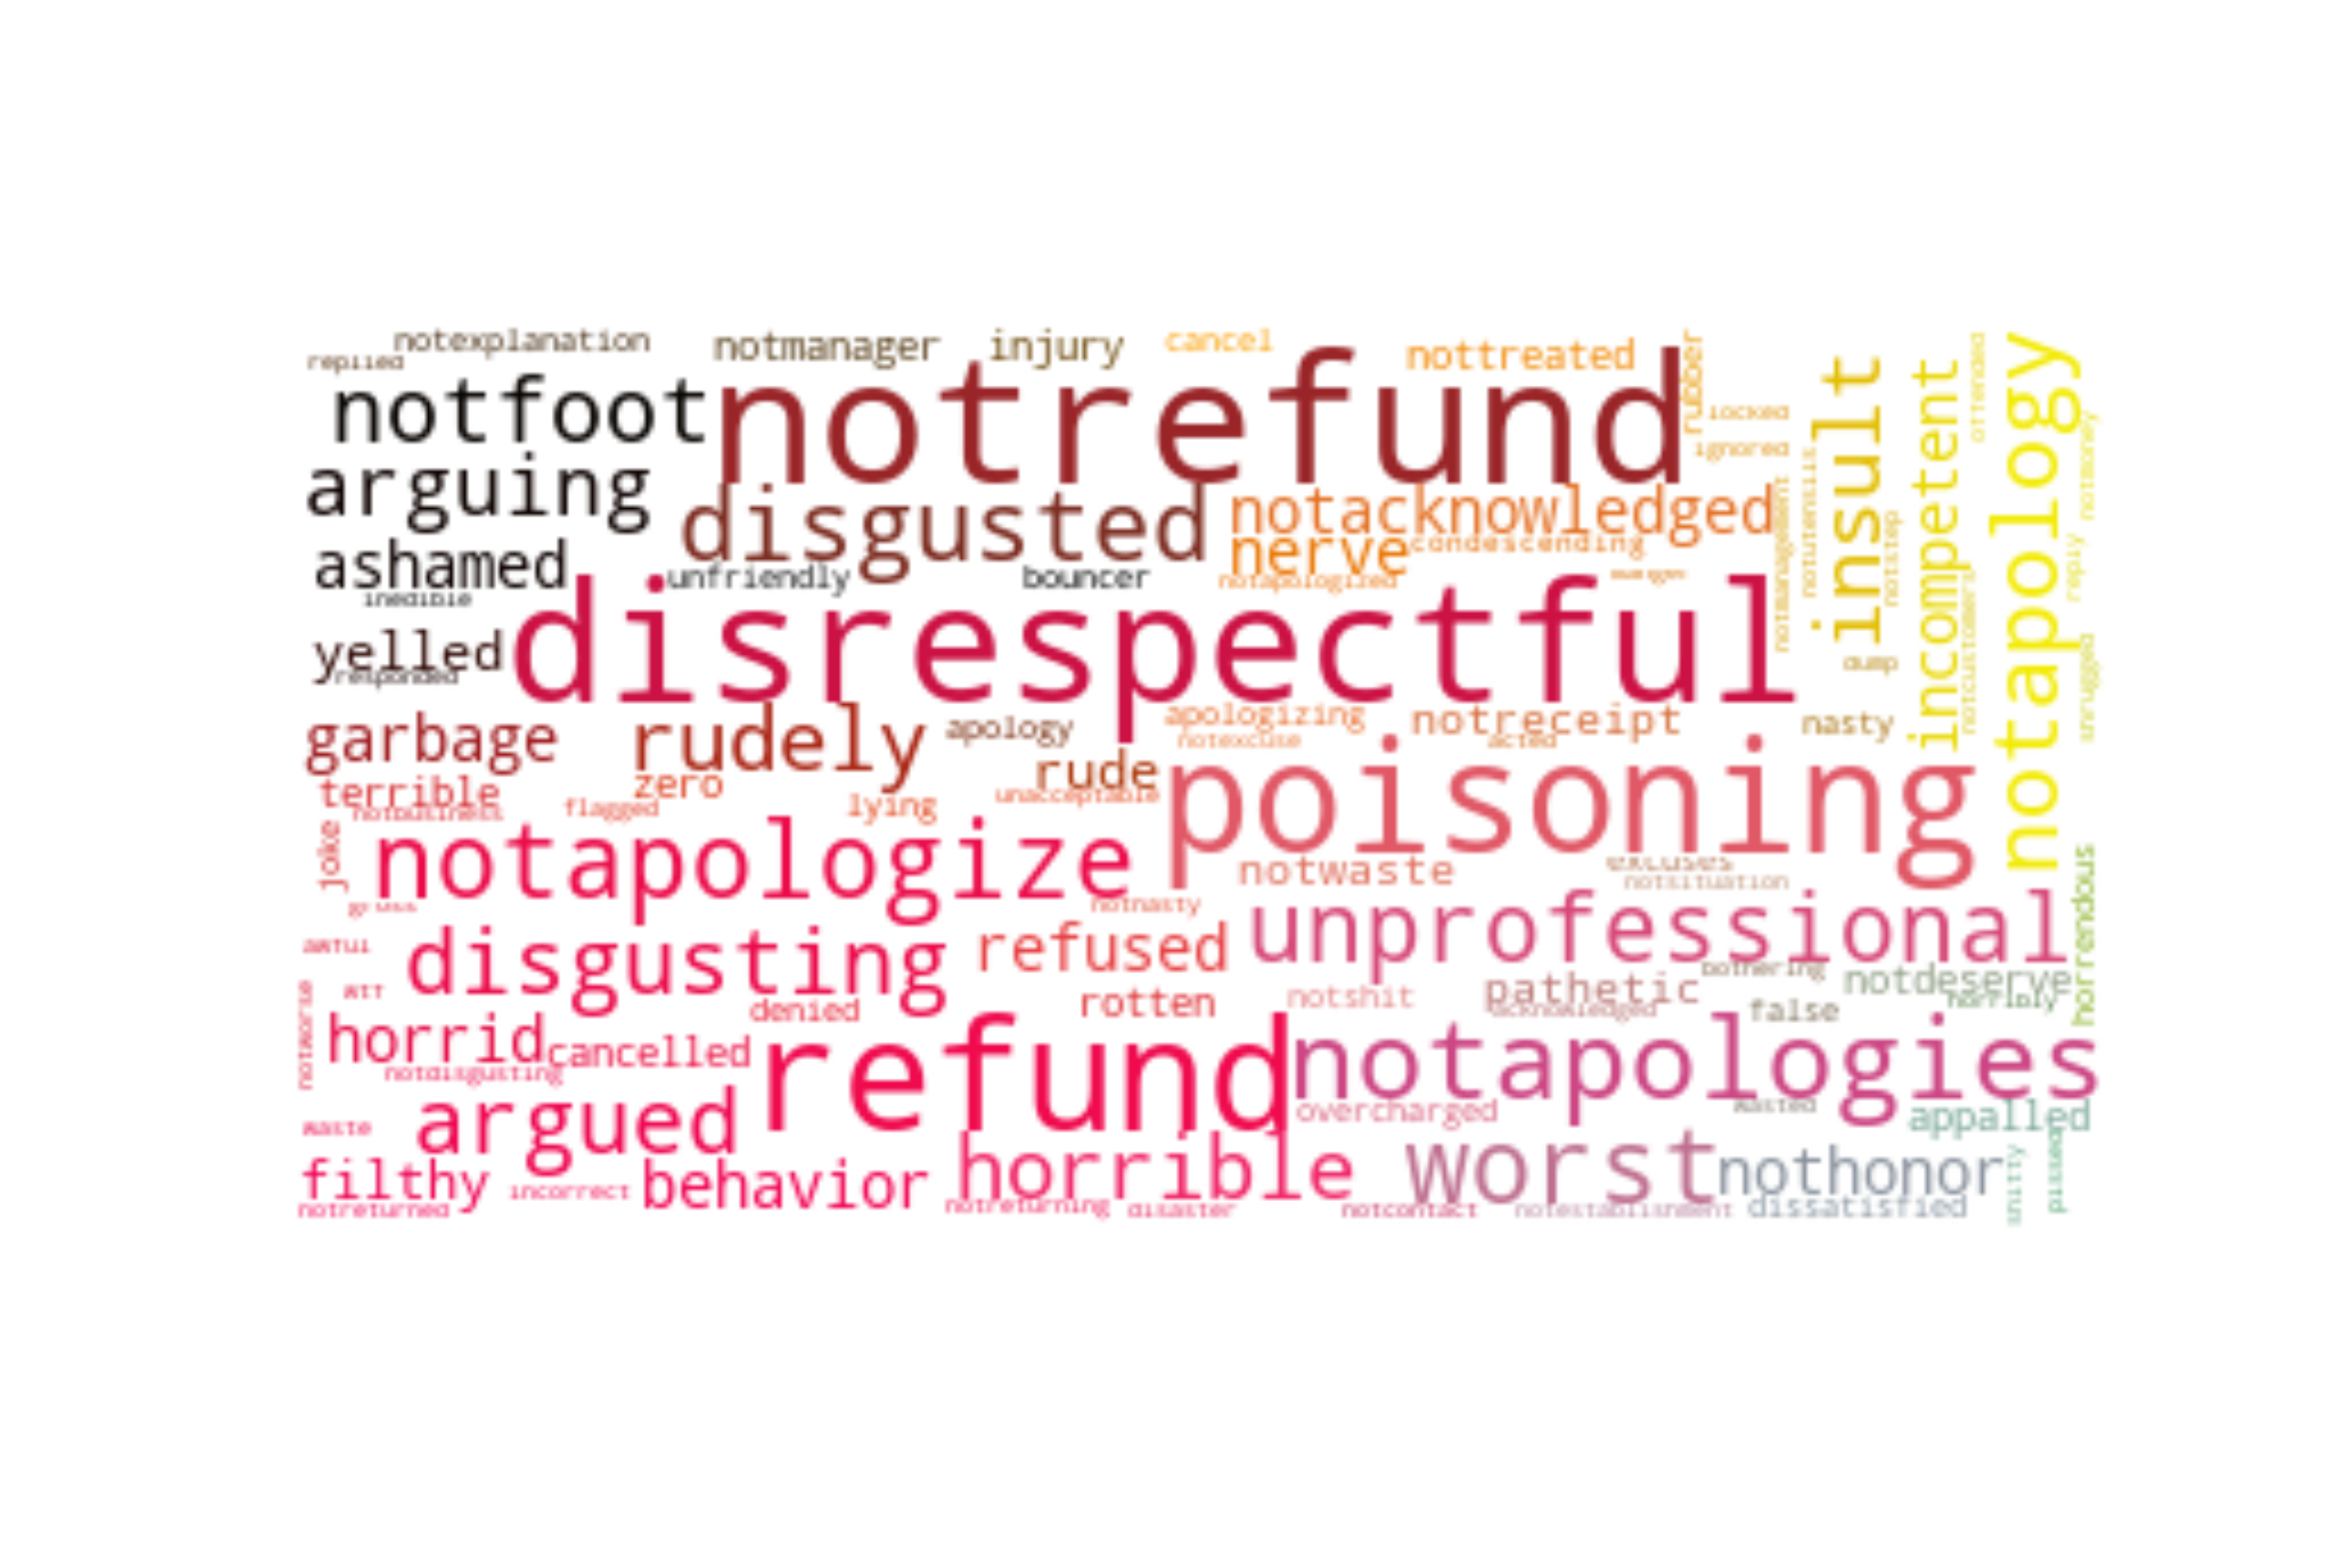
\includegraphics[width=4.8cm,height=5cm]{../image/dist1.png}

\end{minipage}
\end{figure}
\end{frame}

% 3-----------------------------------------------------------------------------------
\begin{frame}{3 Compare MSE with other method}

\begin{table}[]
\centering
\caption*{\huge{MSE} }

\begin{tabular}{lrrrrrr}
Feature$\backslash$ Model &LM    & NB &NN  &LSTM  &GLM  & SVM \\
\hline
vector + ad   & 0.673     & 0.974  & 0.494   & \large\textbf{0.493}  & 0.698    & NA \\
vector        & 0.720     & 1.112  & 0.524   & 0.526  & 0.756    & 0.585  \\
additional            & \textbf{0.836}    & 1.459  & 0.614   & 0.612  & 0.894    & NA  \\
frequence     & NA & 1.126  & 1.210   & NA  & 0.864    & 0.790  \\
tf-idf        & 0.889 & 1.114 & 0.804   & NA  & 0.836    & 0.770  \\
\hline

\end{tabular}
\begin{tablenotes}
	\small
	\item tested on 100000 data
\end{tablenotes}

\end{table}

\end{frame}

% 4----------------------------------------------------------------------------------
\begin{frame}{4 Interpretable Model}
$$
\begin{aligned}
\hat{y} &=3.65+0.04* scale(year)+0.04*loc1+0.06*loc2\\
&-0.11*S1-0.17*S2-0.03*S3+0.03*S4+0.14*S5
\end{aligned}
$$


\end{frame}


\begin{frame}{5 Strengths and Weaknesses}
\textbf{Strengths} \\
RMSE 0.635 for best model feature combination prediction\\
 Inclusion of additional informative variables contributes to the reduction of MSE by 0.033
 \newline
 \newline
\textbf{Weaknesses}\\
Grid search over various model parameters 
\end{frame}

\begin{frame}
\Huge{\centerline{Thank You!}}
\end{frame}
\end{document}
